\section{Ejercicio 1: Conexión a datos de Power BI - Tarea 3: Forma de Datos} 

1. In the Fields pane, right-click Query1, click Rename, type Customers, and then press Enter.\\

	\begin{center}
	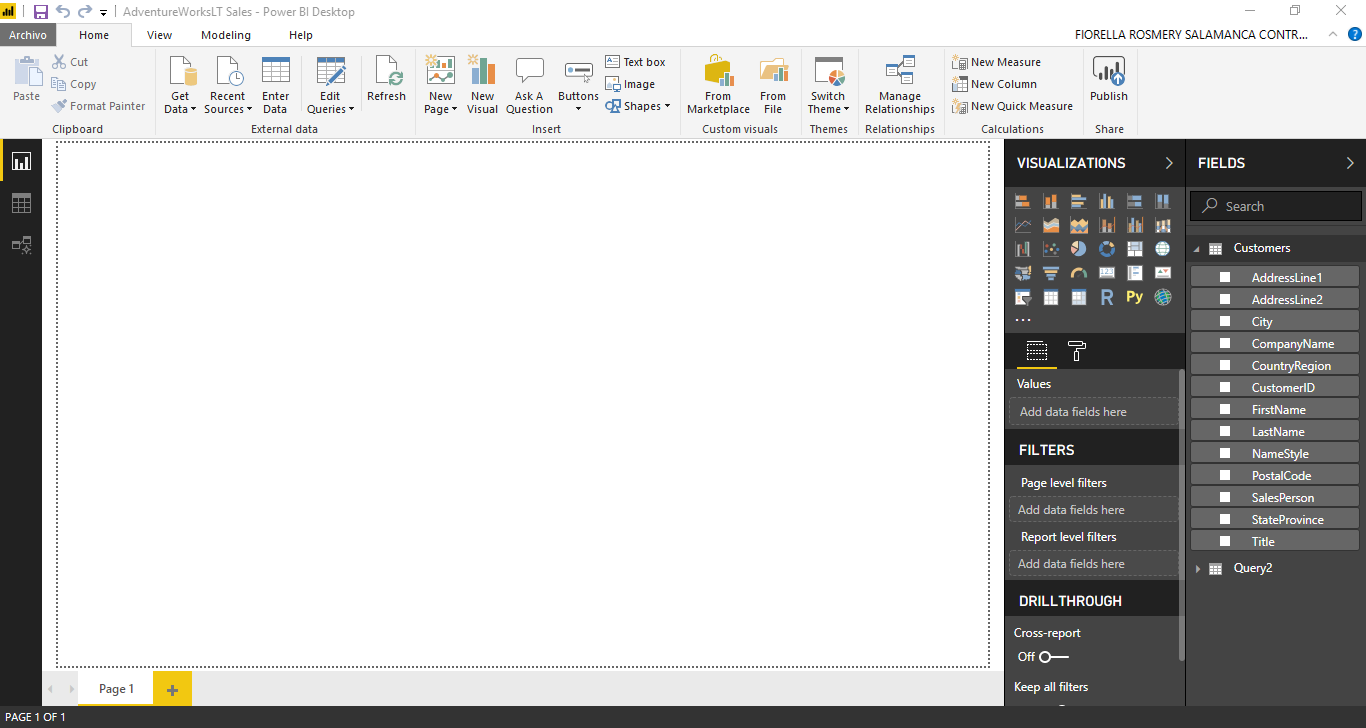
\includegraphics[width=17cm]{./Imagenes/Ejercicio1/Tarea3/1}
	\end{center}	

2. Right-click Query2, click Rename, type Sales, and then press Enter.\\

	\begin{center}
	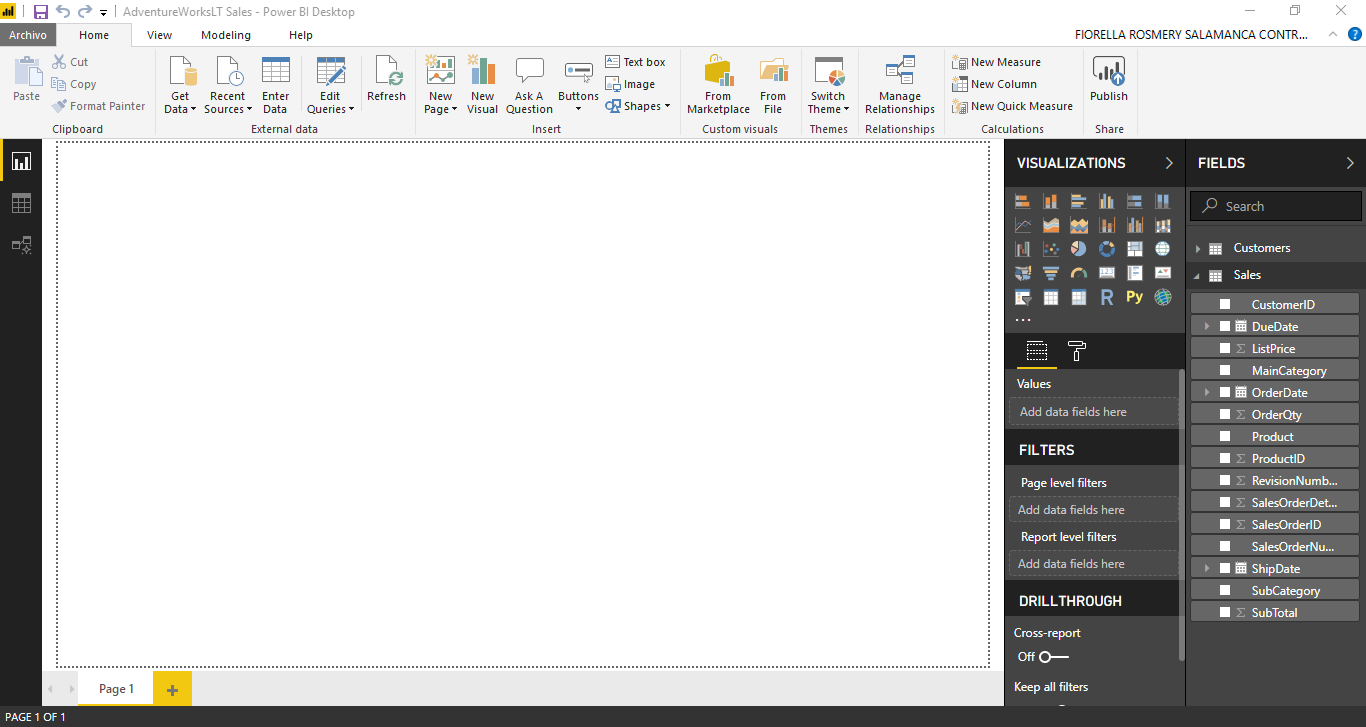
\includegraphics[width=17cm]{./Imagenes/Ejercicio1/Tarea3/2}
	\end{center}	

3. Expand the two tables to display all of the fields.\\
4. In the left navigation bar, click Data.\\
5. In the Fields pane, click the Customers table, if it is not already selected.\\
6. Right-click the NameStyle column, and click Delete.\\

	\begin{center}
	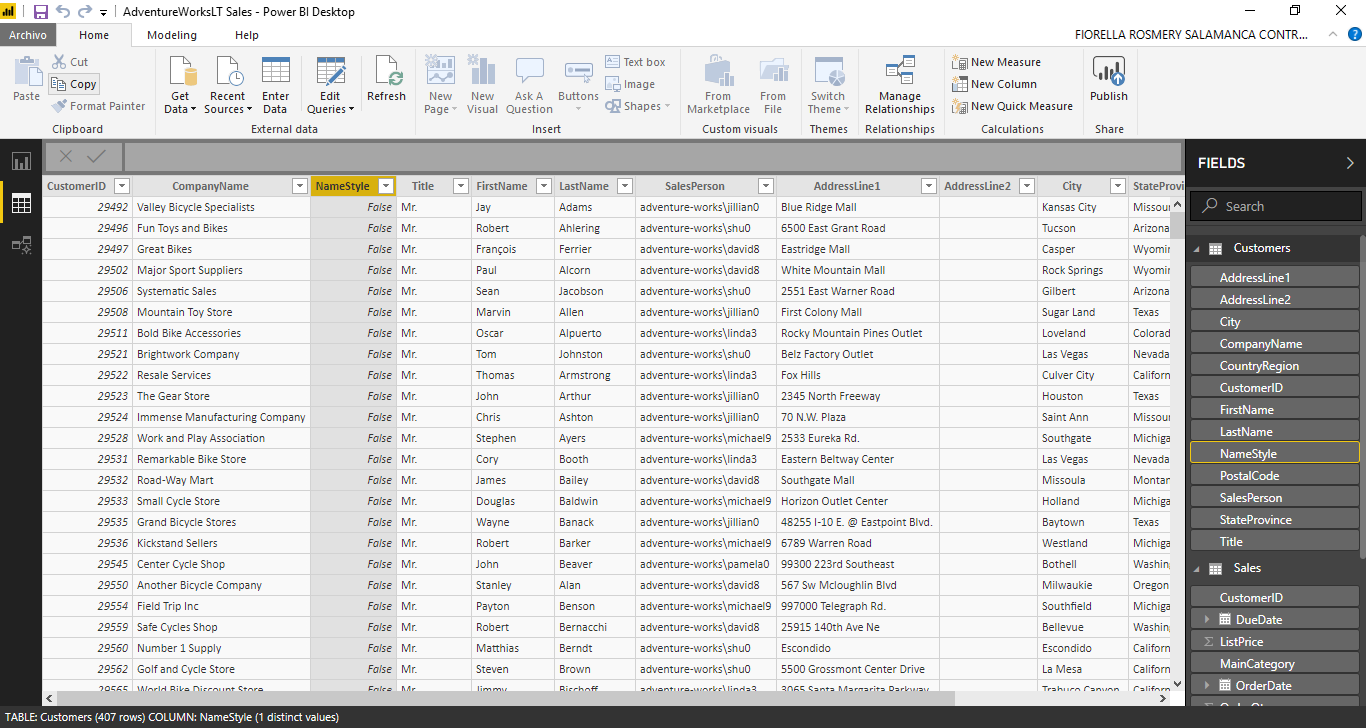
\includegraphics[width=17cm]{./Imagenes/Ejercicio1/Tarea3/3}
	\end{center}	

7. In the Delete Column dialog box, click Delete.\\

	\begin{center}
	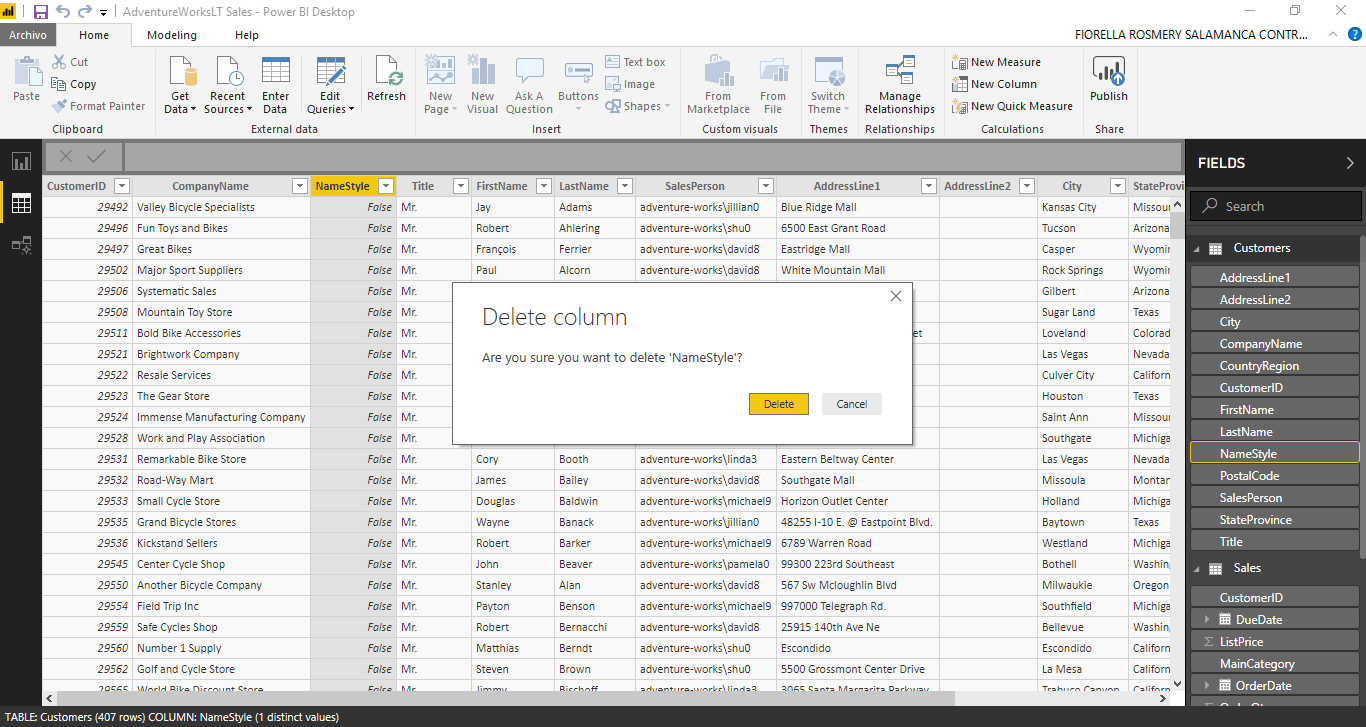
\includegraphics[width=17cm]{./Imagenes/Ejercicio1/Tarea3/4}
	\end{center}	

8. Right-click the SalesPerson column, and click Delete.\\

	\begin{center}
	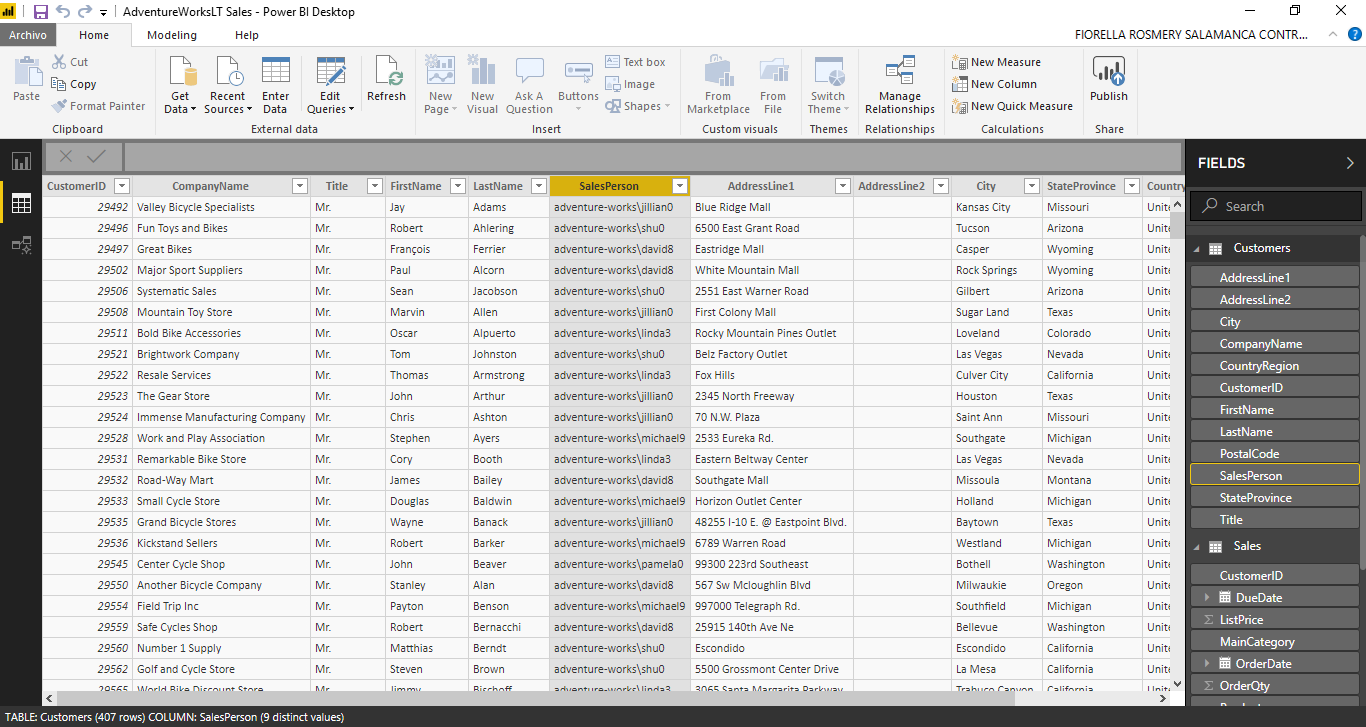
\includegraphics[width=17cm]{./Imagenes/Ejercicio1/Tarea3/5}
	\end{center}	

9. In the Delete Column dialog box, click Delete.\\

	\begin{center}
	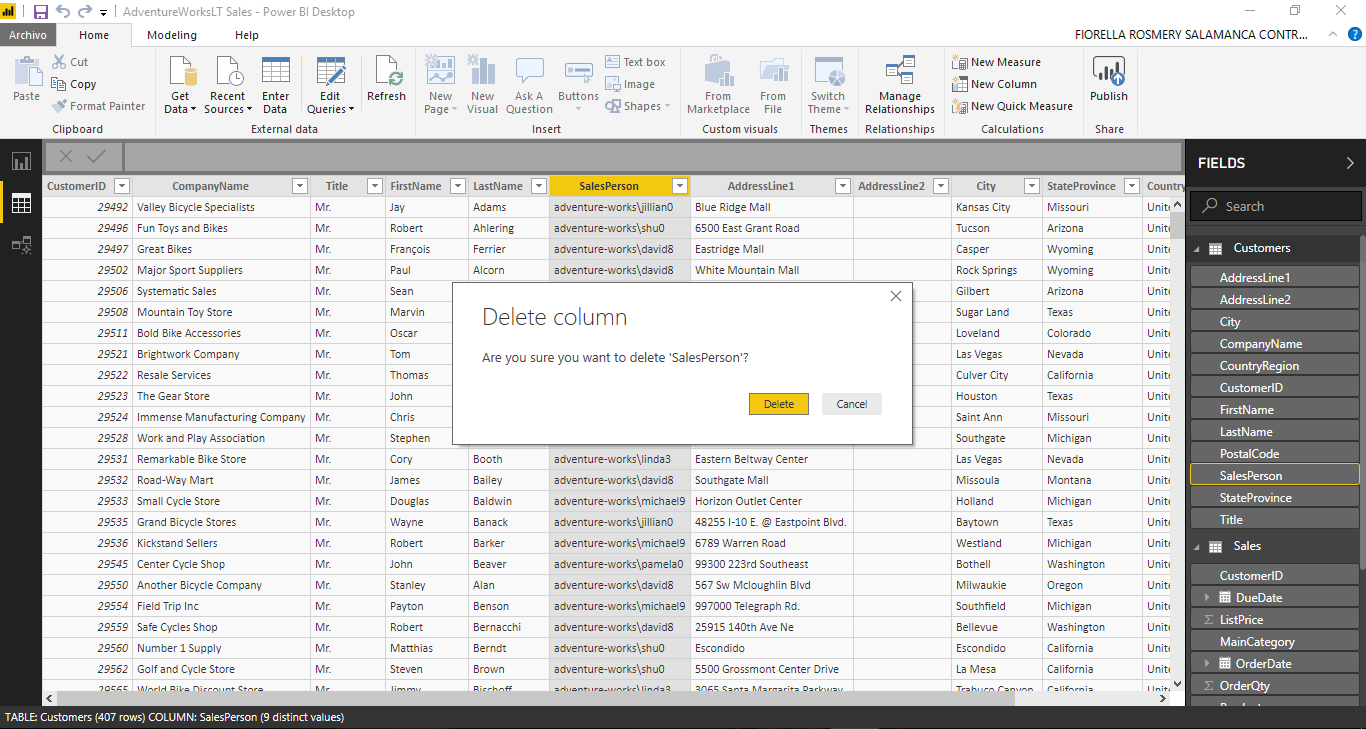
\includegraphics[width=17cm]{./Imagenes/Ejercicio1/Tarea3/6}
	\end{center}	

10. Right-click the CustomerID column, and then click Hide in Report View.\\

	\begin{center}
	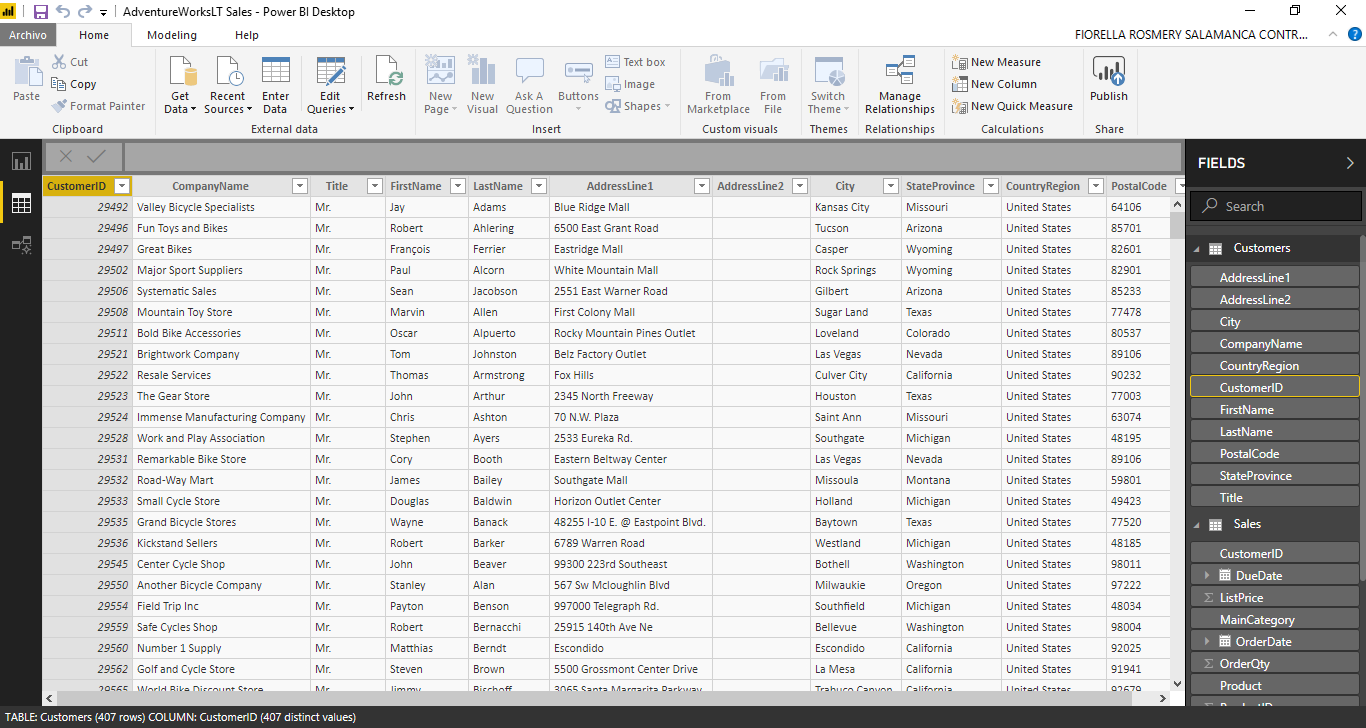
\includegraphics[width=17cm]{./Imagenes/Ejercicio1/Tarea3/7}
	\end{center}	

	\begin{center}
	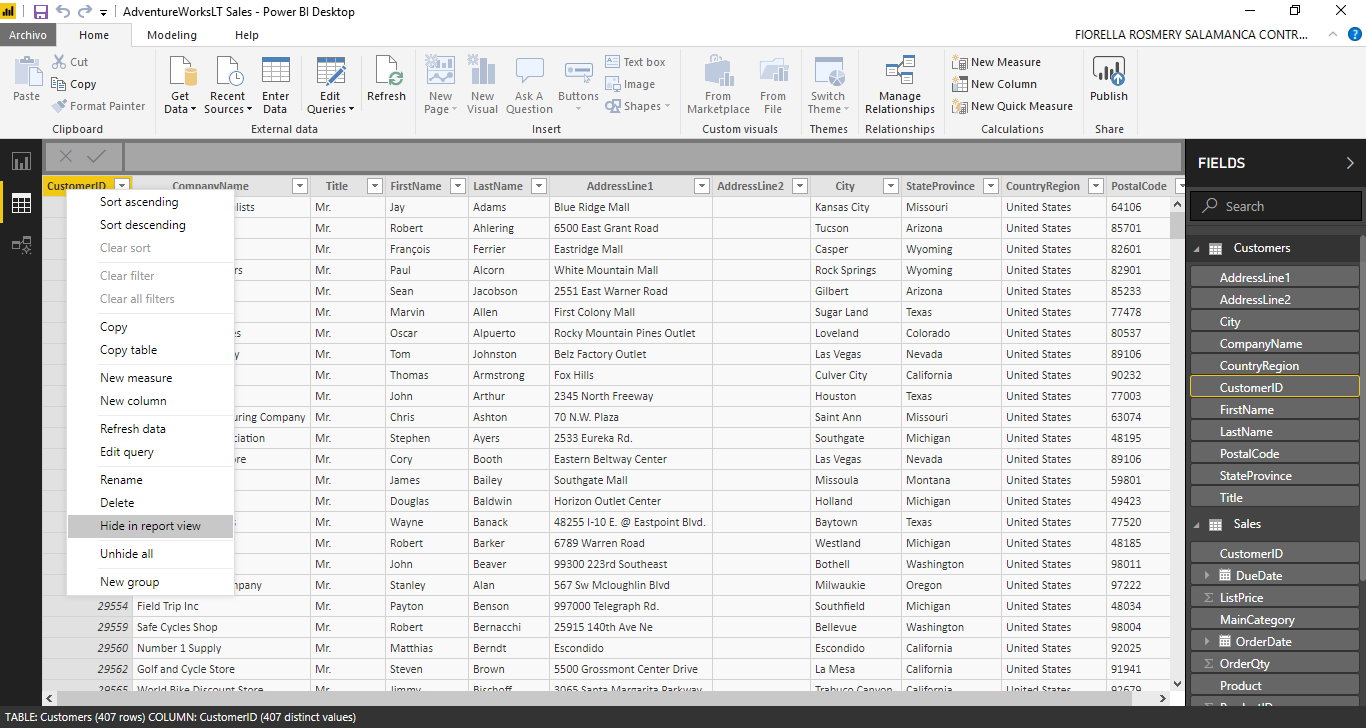
\includegraphics[width=17cm]{./Imagenes/Ejercicio1/Tarea3/8}
	\end{center}	

11. Click the AddressLine1 column header.\\

	\begin{center}
	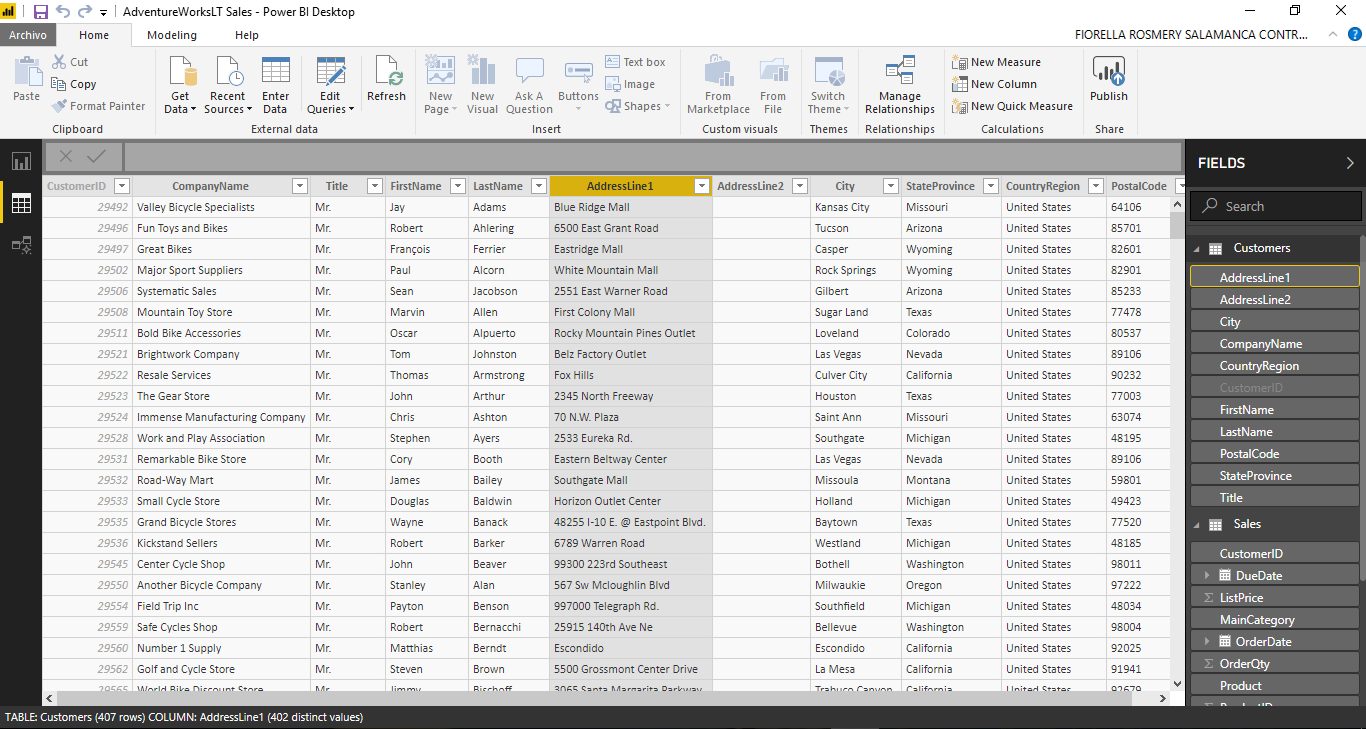
\includegraphics[width=17cm]{./Imagenes/Ejercicio1/Tarea3/9}
	\end{center}	

12. On the Modeling ribbon, in the Properties group, click Data Category: Uncategorized, and then click Address.\\

	\begin{center}
	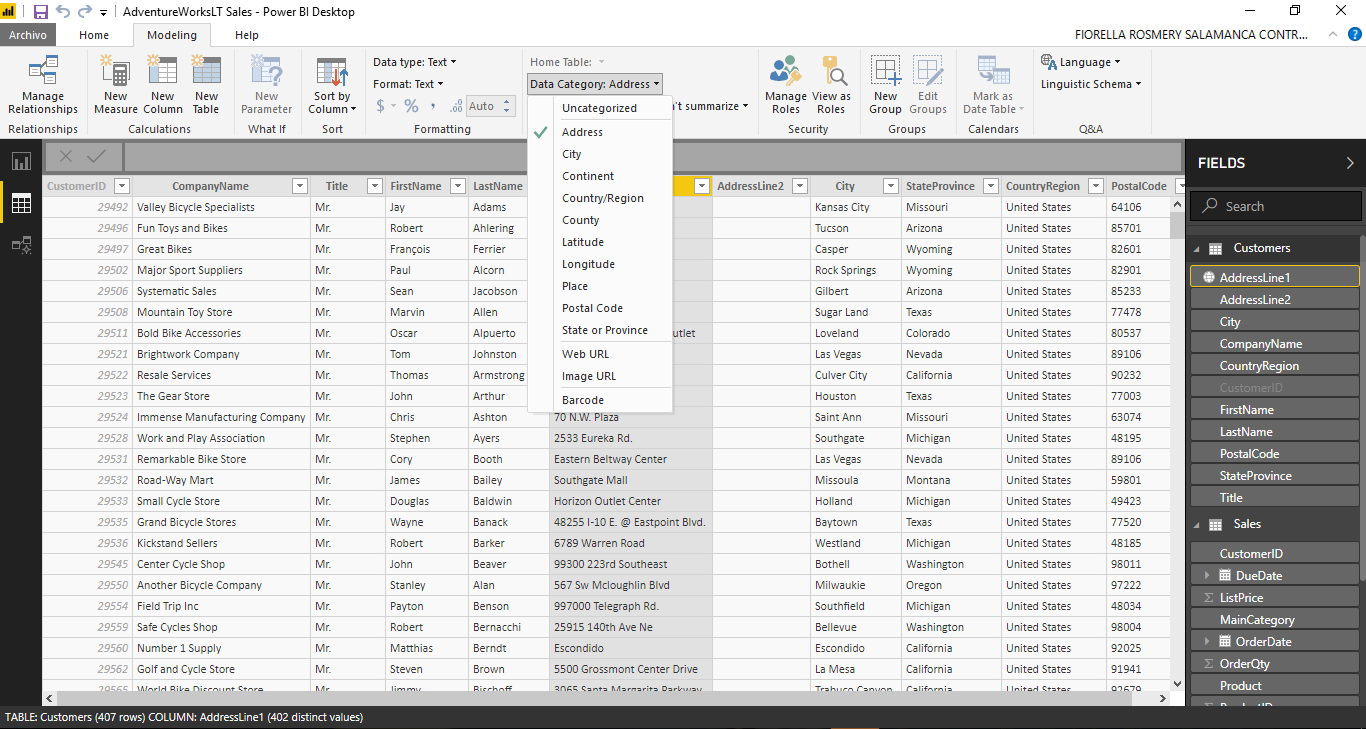
\includegraphics[width=17cm]{./Imagenes/Ejercicio1/Tarea3/10}
	\end{center}	

13. Click the City column header.\\

	\begin{center}
	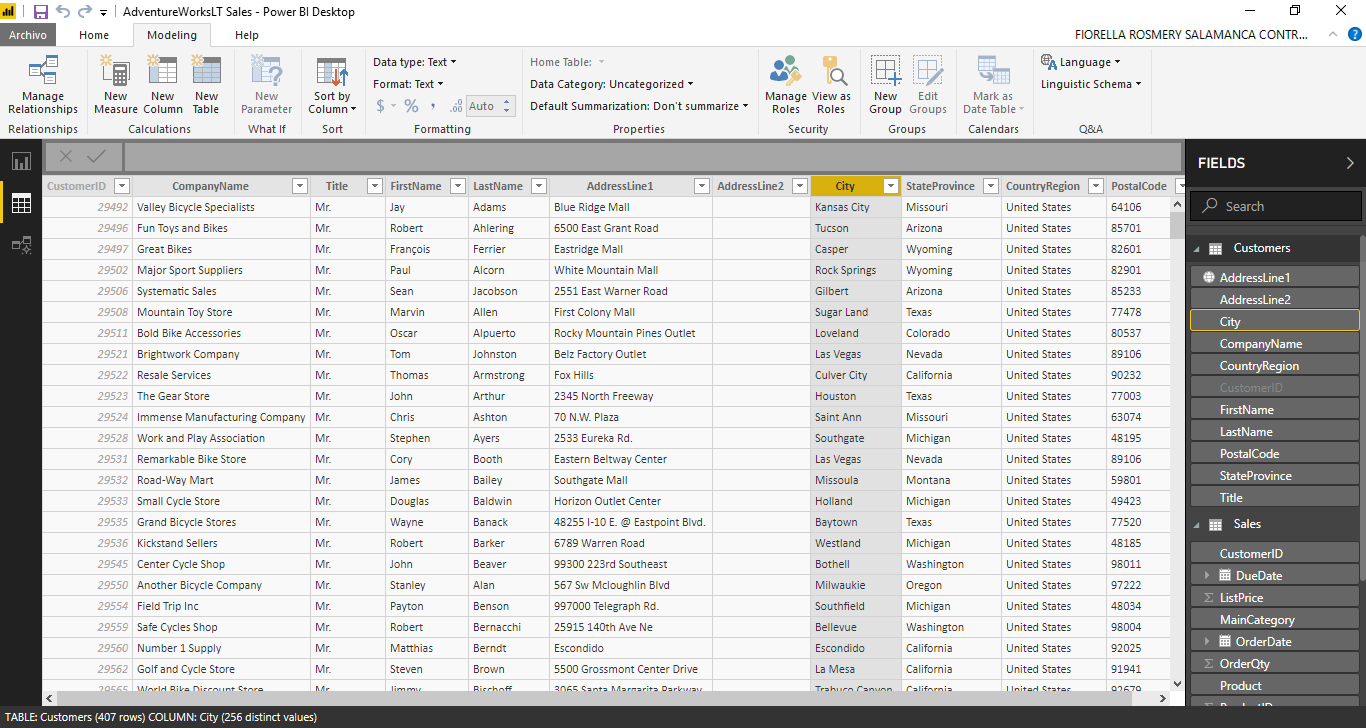
\includegraphics[width=17cm]{./Imagenes/Ejercicio1/Tarea3/11}
	\end{center}	

14. On the Modeling ribbon, in the Properties group, click Data Category: Uncategorized, and then click City.\\

	\begin{center}
	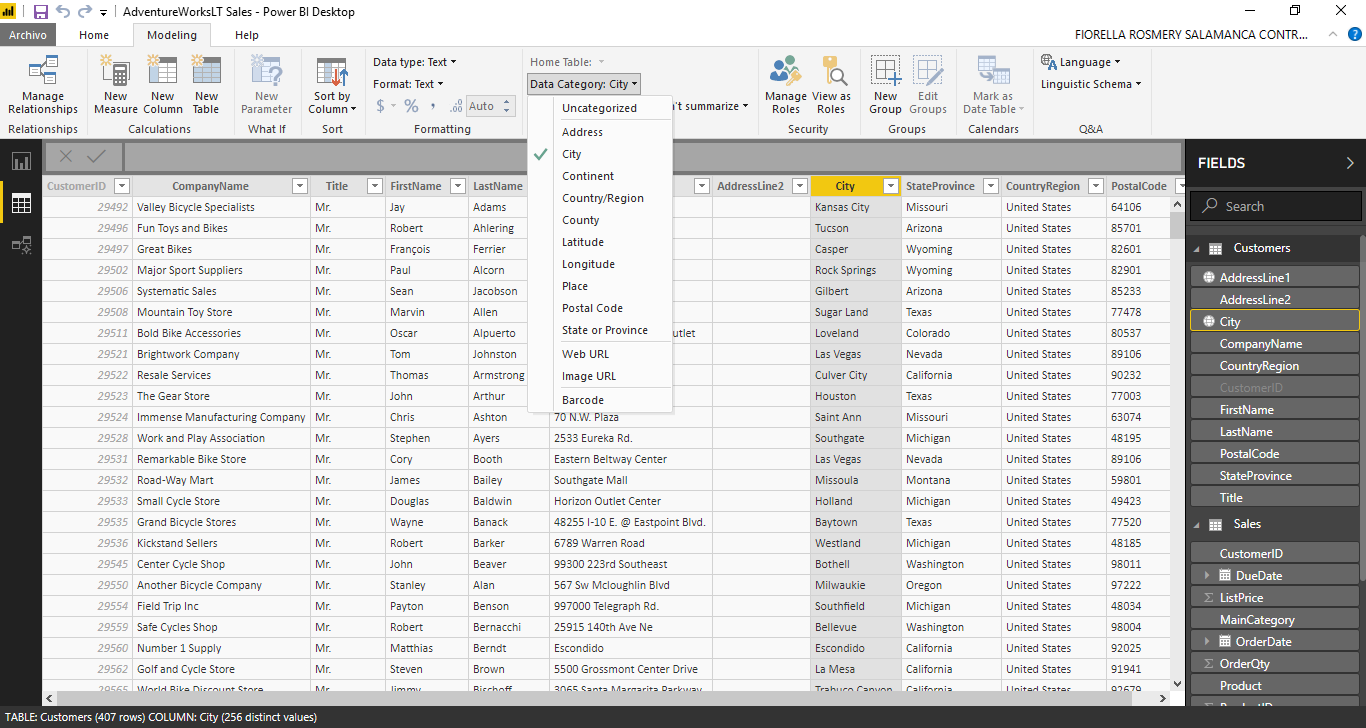
\includegraphics[width=17cm]{./Imagenes/Ejercicio1/Tarea3/12}
	\end{center}	

15. Click the StateProvince column header.\\

	\begin{center}
	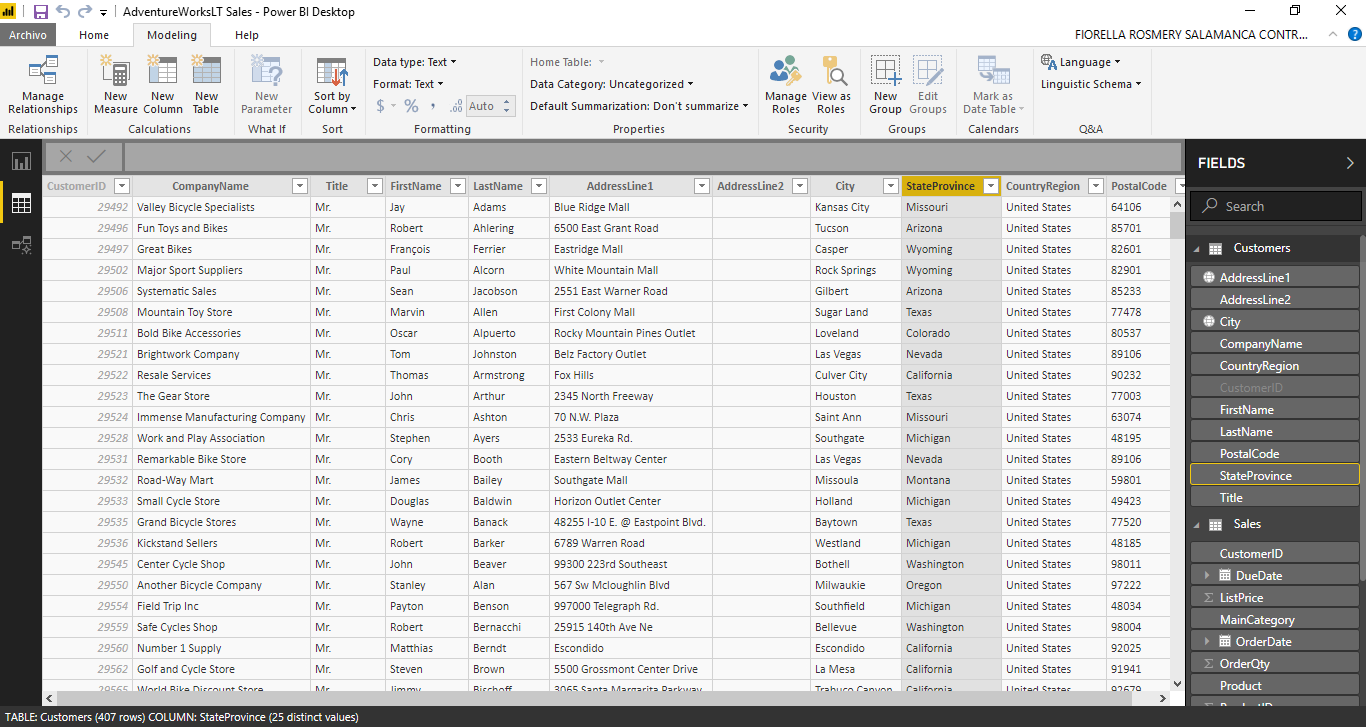
\includegraphics[width=17cm]{./Imagenes/Ejercicio1/Tarea3/13}
	\end{center}	

16. On the Modeling ribbon, in the Properties group, click Data Category: Uncategorized, and then click State or Province.\\

	\begin{center}
	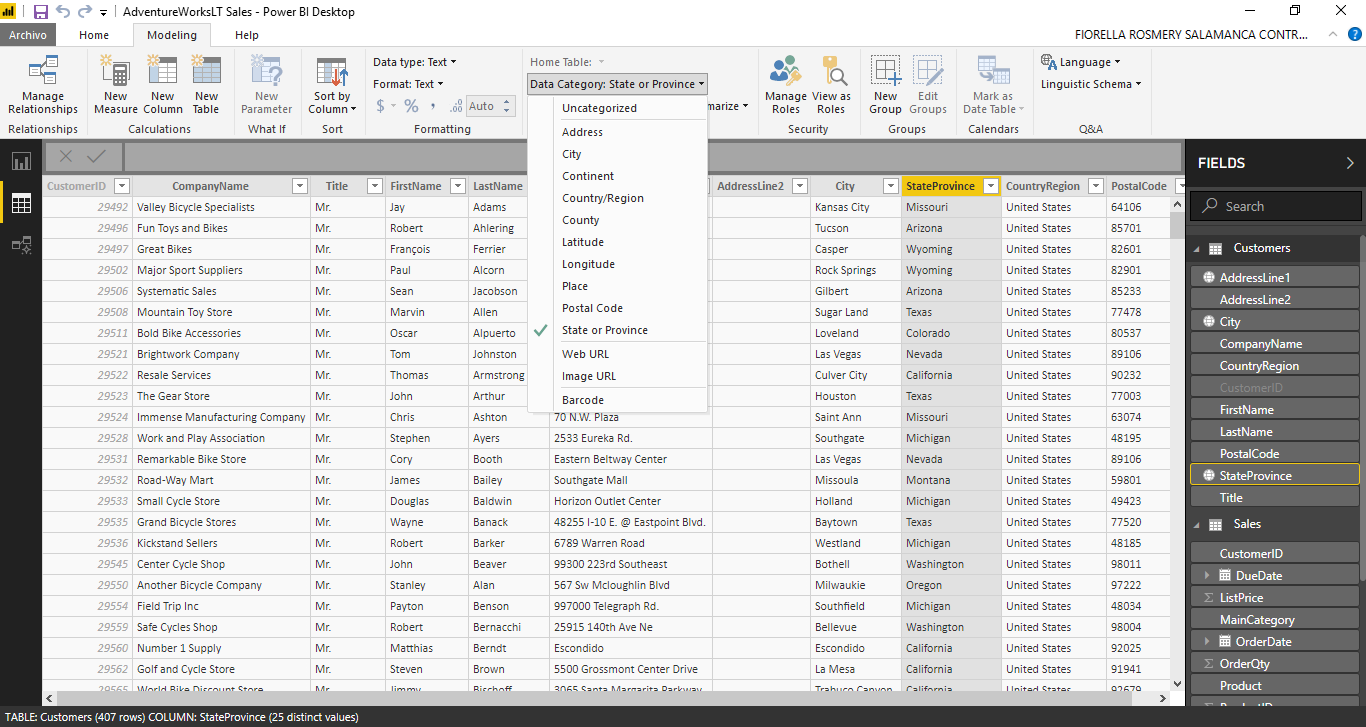
\includegraphics[width=17cm]{./Imagenes/Ejercicio1/Tarea3/14}
	\end{center}	

17. Click the CountryRegion column header.\\

	\begin{center}
	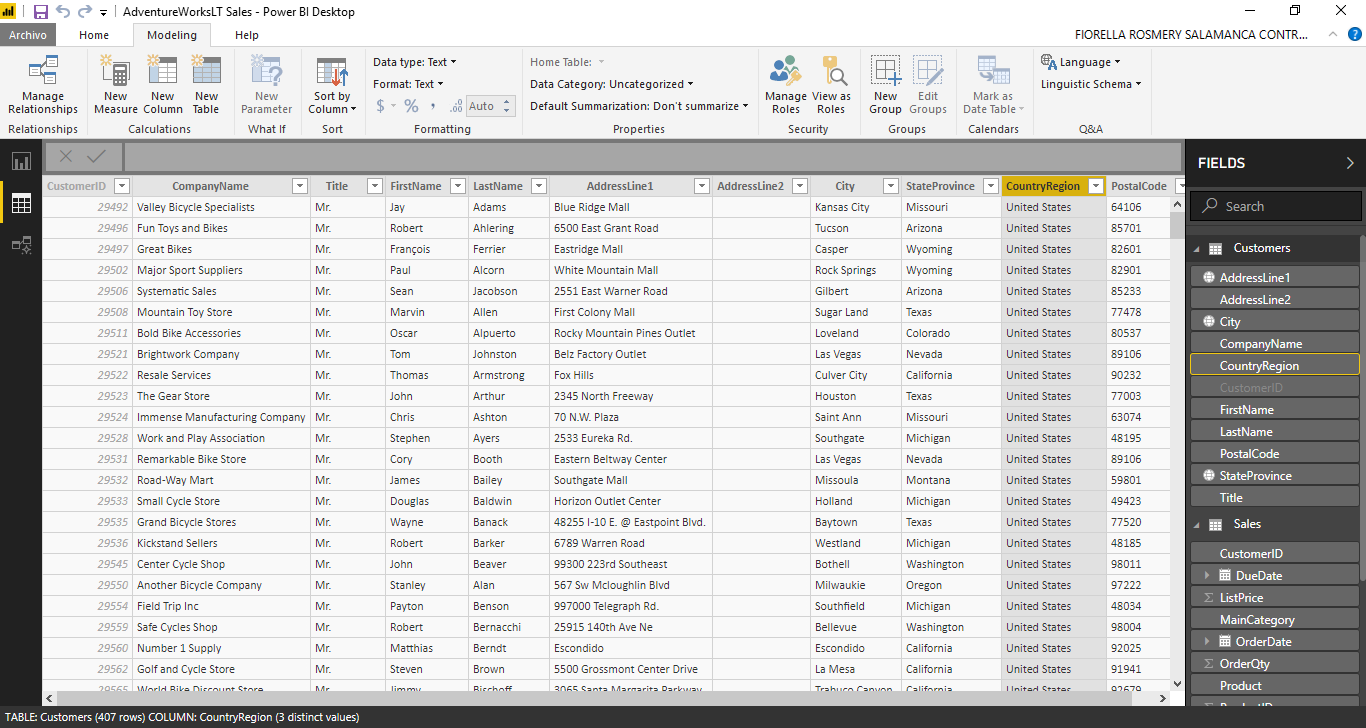
\includegraphics[width=17cm]{./Imagenes/Ejercicio1/Tarea3/15}
	\end{center}	

18. On the Modeling ribbon, in the Properties group, click Data Category: Uncategorized, and then click Country/Region.\\

	\begin{center}
	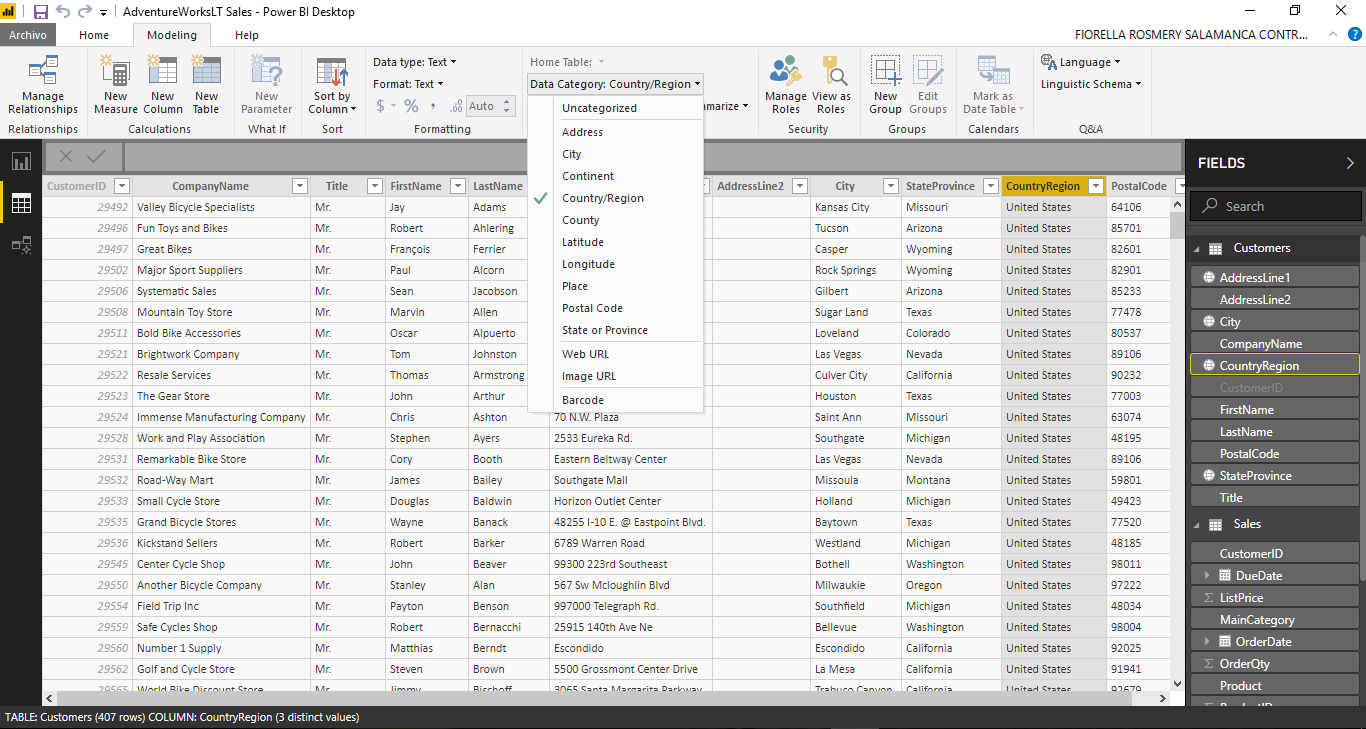
\includegraphics[width=17cm]{./Imagenes/Ejercicio1/Tarea3/16}
	\end{center}	

19. Click the PostalCode column header.\\

	\begin{center}
	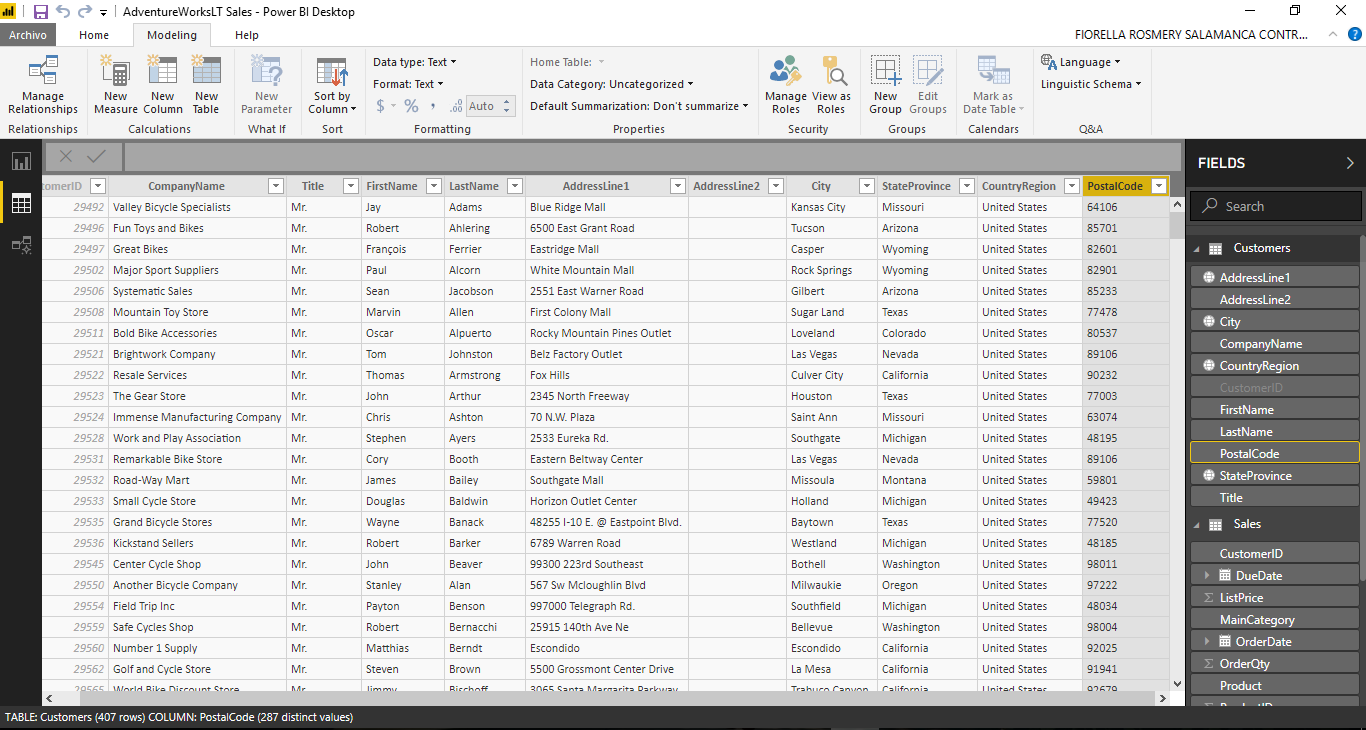
\includegraphics[width=17cm]{./Imagenes/Ejercicio1/Tarea3/17}
	\end{center}	

20. On the Modeling ribbon, in the Properties group, click Data Category: Uncategorized, and then click Postal Code.\\

	\begin{center}
	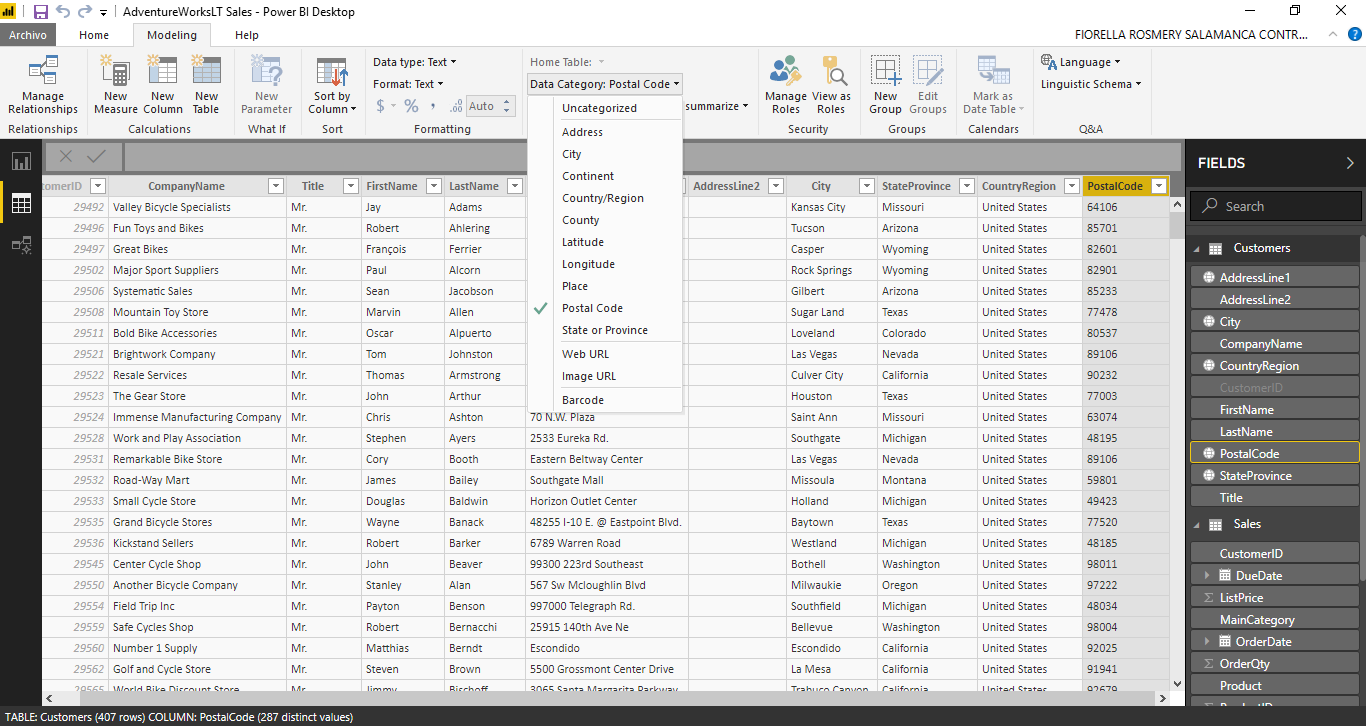
\includegraphics[width=17cm]{./Imagenes/Ejercicio1/Tarea3/18}
	\end{center}	

21. On the Modeling ribbon, in the Calculations group, click New Column, and then in the formula bar, type the following expression and press Enter:\\

\textbf{FullAddress = Customers[AddressLine1] \& ", " \& Customers[City] \& ", " \&
Customers[StateProvince] \& ", " \& Customers[CountryRegion] \& ", " \&
Customers[PostalCode]} 

	\begin{center}
	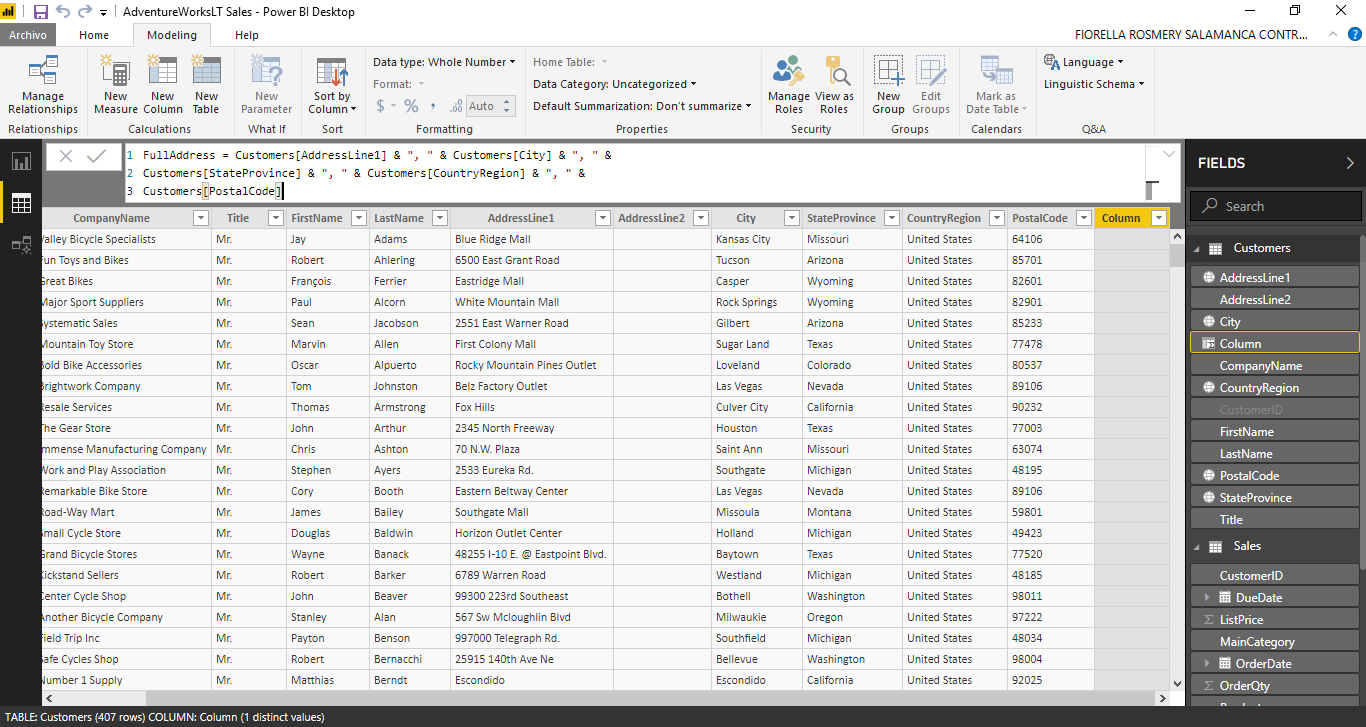
\includegraphics[width=17cm]{./Imagenes/Ejercicio1/Tarea3/19}
	\end{center}	

22. In the Fields pane, click Sales.\\

	\begin{center}
	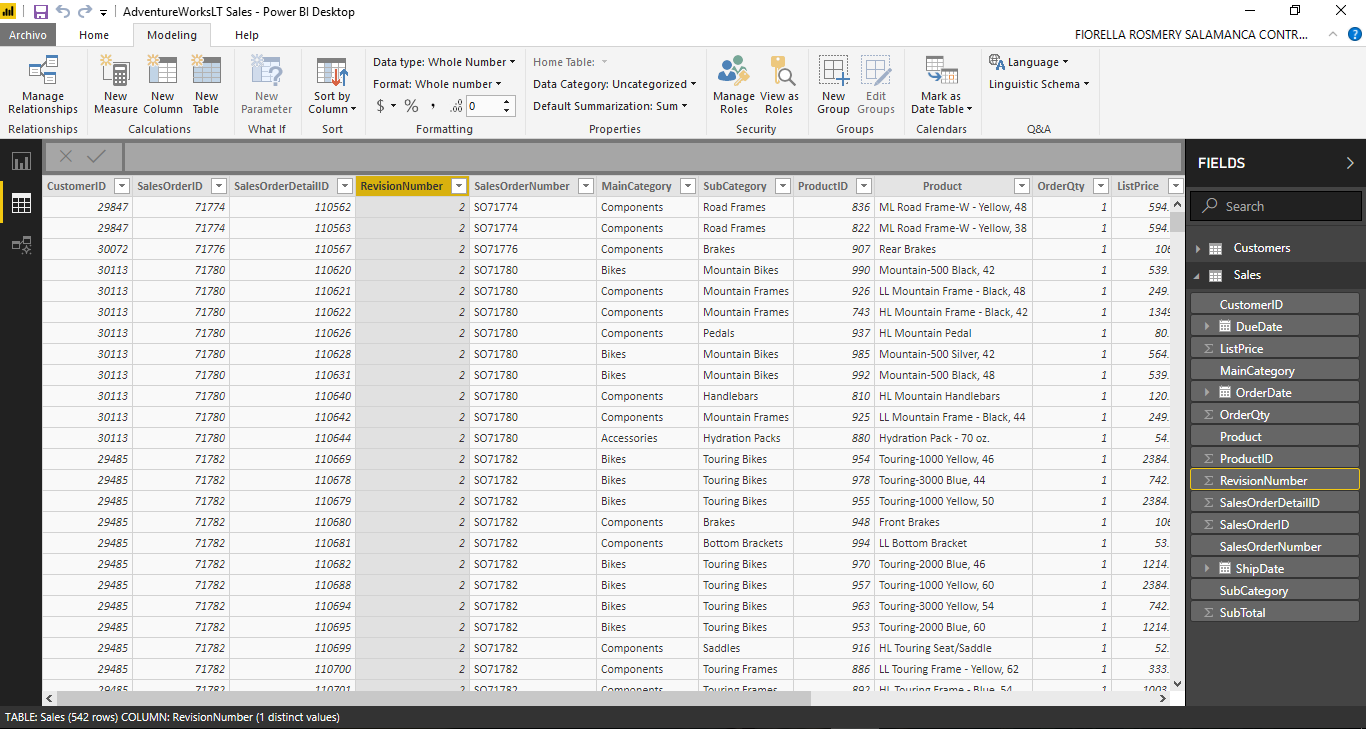
\includegraphics[width=17cm]{./Imagenes/Ejercicio1/Tarea3/20}
	\end{center}	

23. Right-click the RevisionNumber column, and click Delete.\\
24. In the Delete Column dialog box, click Delete.\\

	\begin{center}
	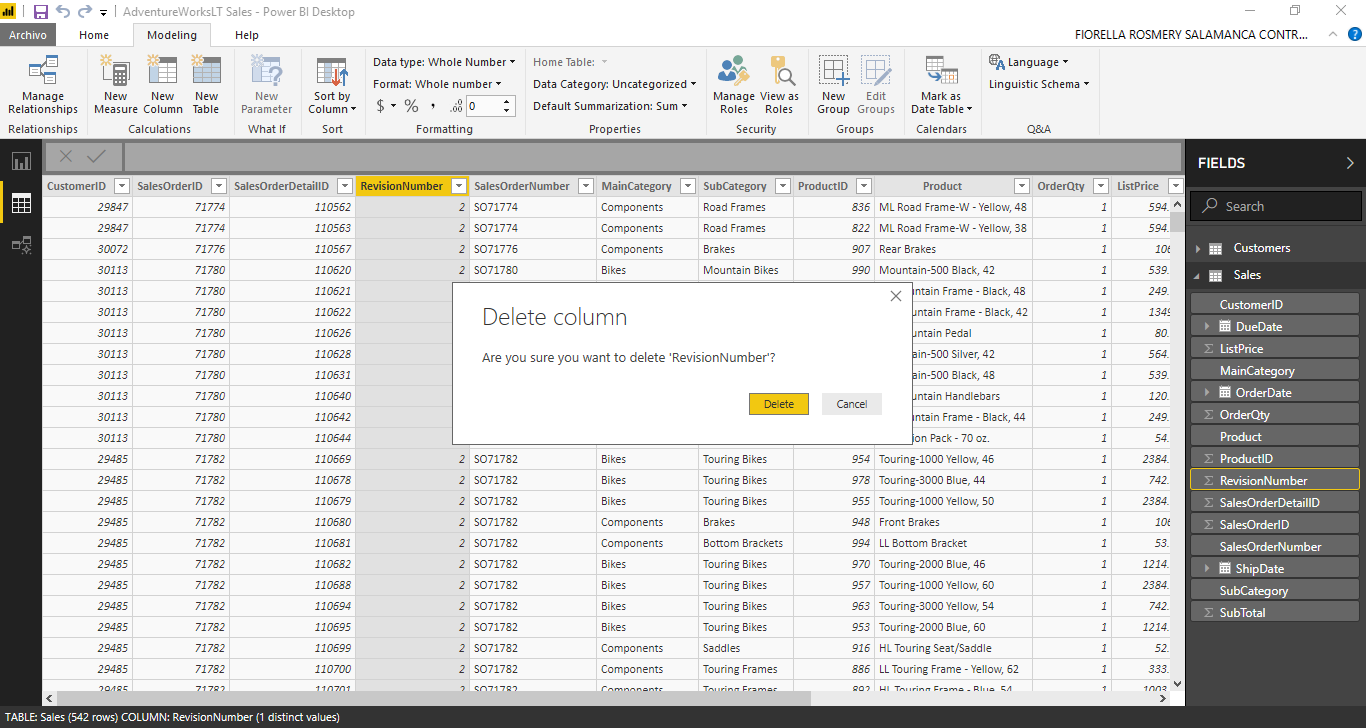
\includegraphics[width=17cm]{./Imagenes/Ejercicio1/Tarea3/21}
	\end{center}	

25. Right-click the SalesOrderNumber column, and click Delete.\\

	\begin{center}
	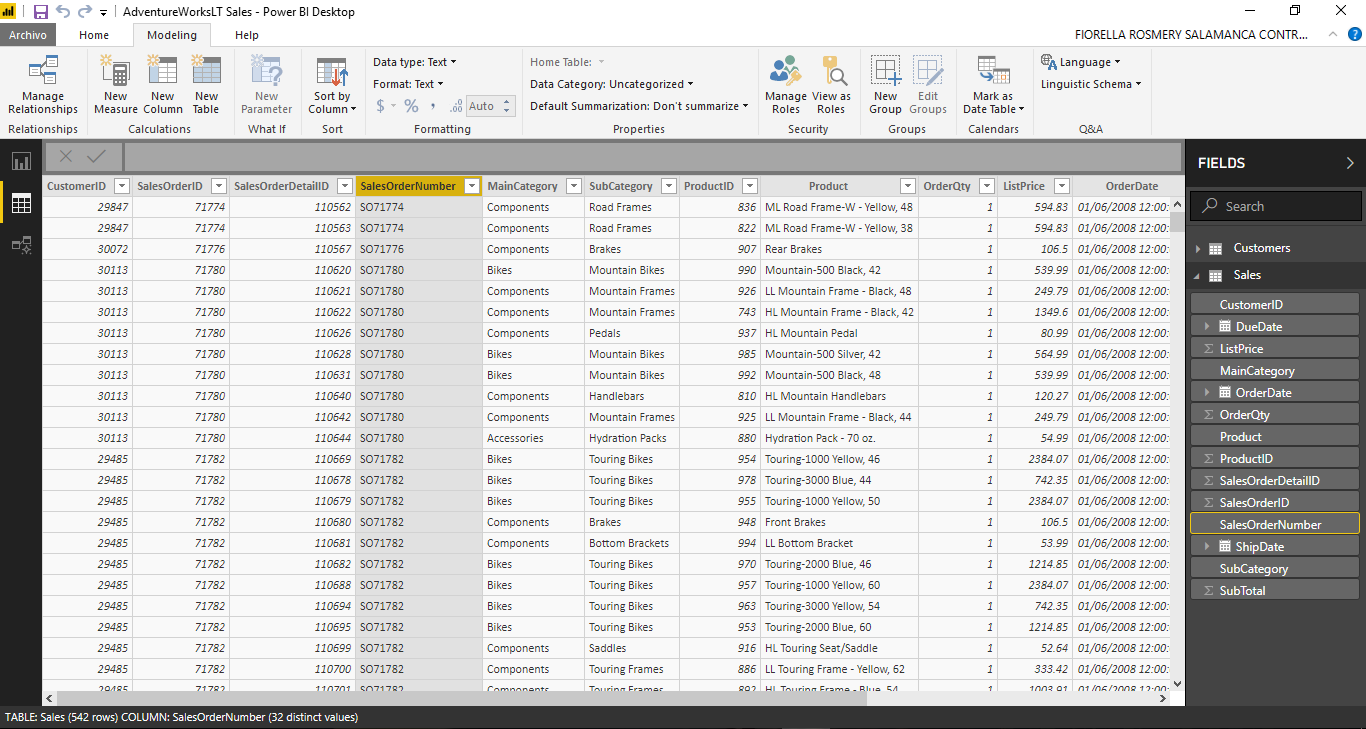
\includegraphics[width=17cm]{./Imagenes/Ejercicio1/Tarea3/22}
	\end{center}	

26. In the Delete Column dialog box, click Delete.\\

	\begin{center}
	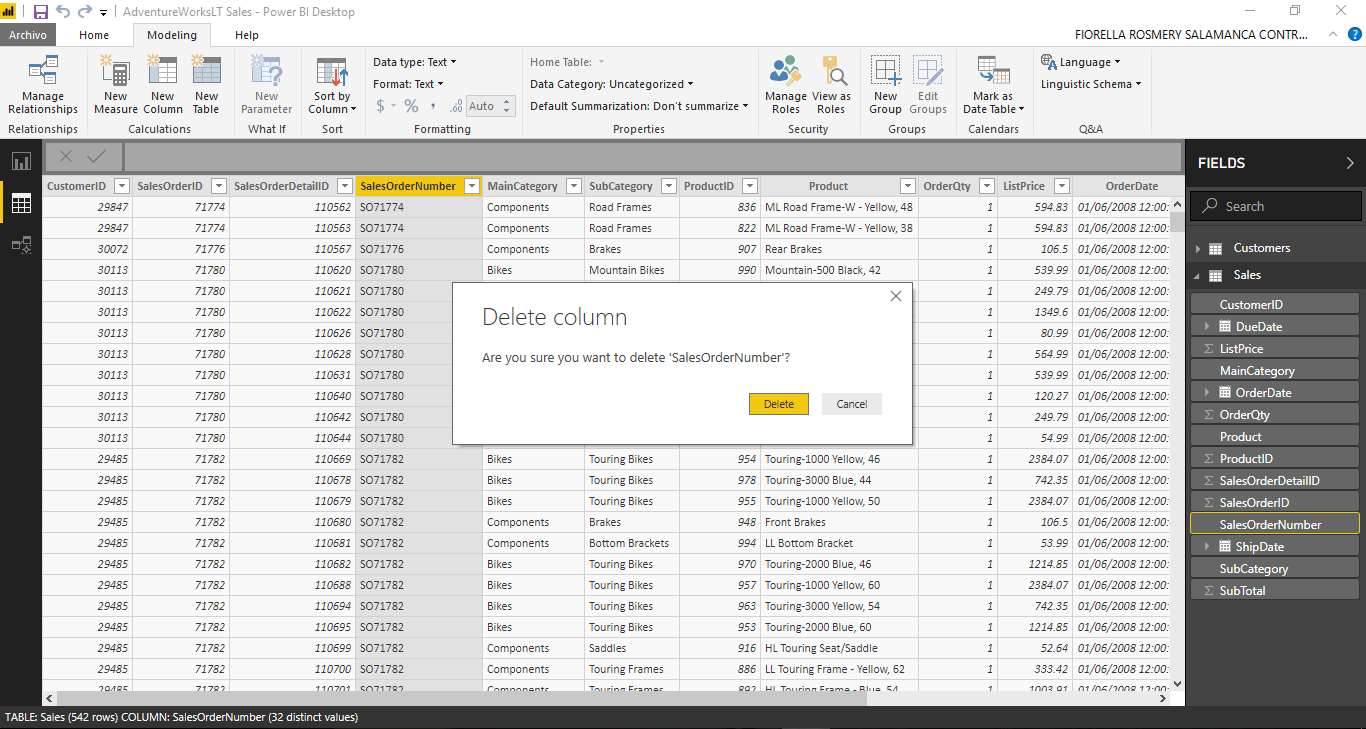
\includegraphics[width=17cm]{./Imagenes/Ejercicio1/Tarea3/23}
	\end{center}	

27. Right-click the CustomerID column, and then click Hide in Report View.\\

	\begin{center}
	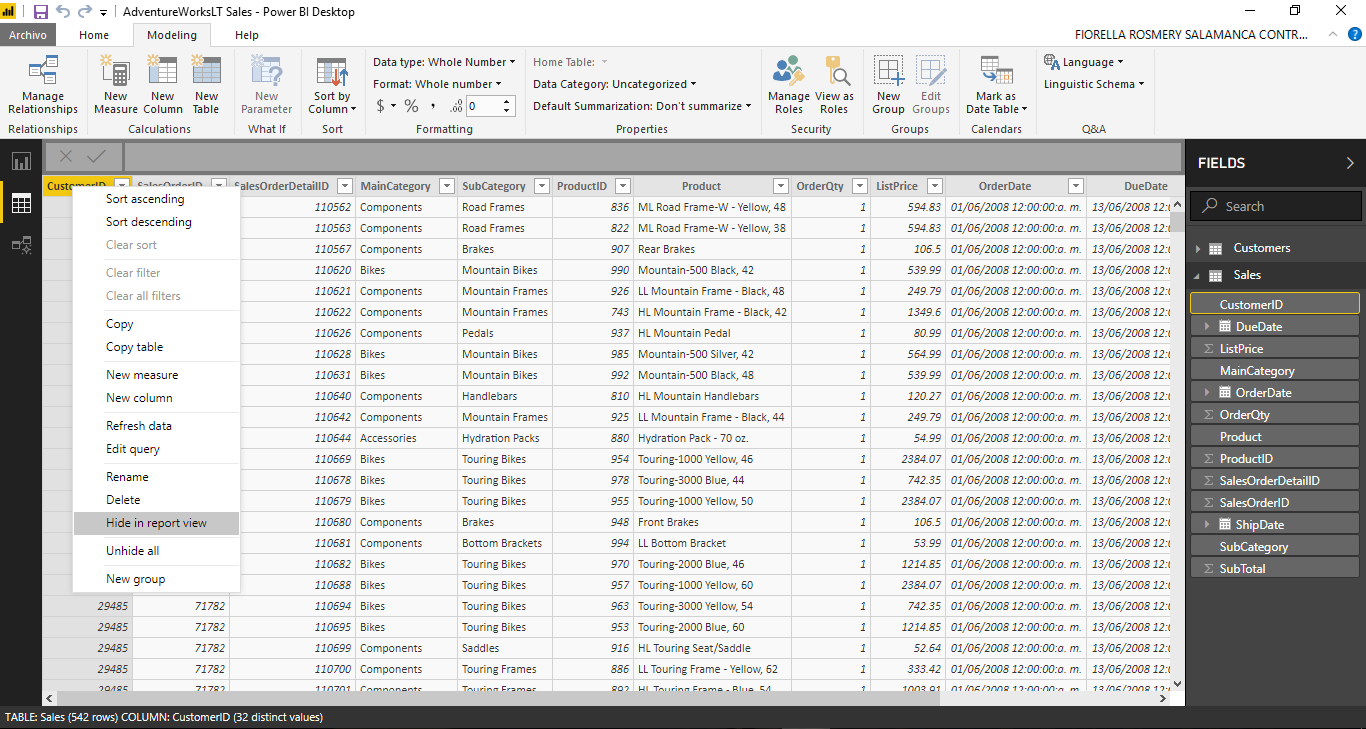
\includegraphics[width=17cm]{./Imagenes/Ejercicio1/Tarea3/24}
	\end{center}	

28. Right-click the SalesOrderID column, and then click Hide in Report View.\\

	\begin{center}
	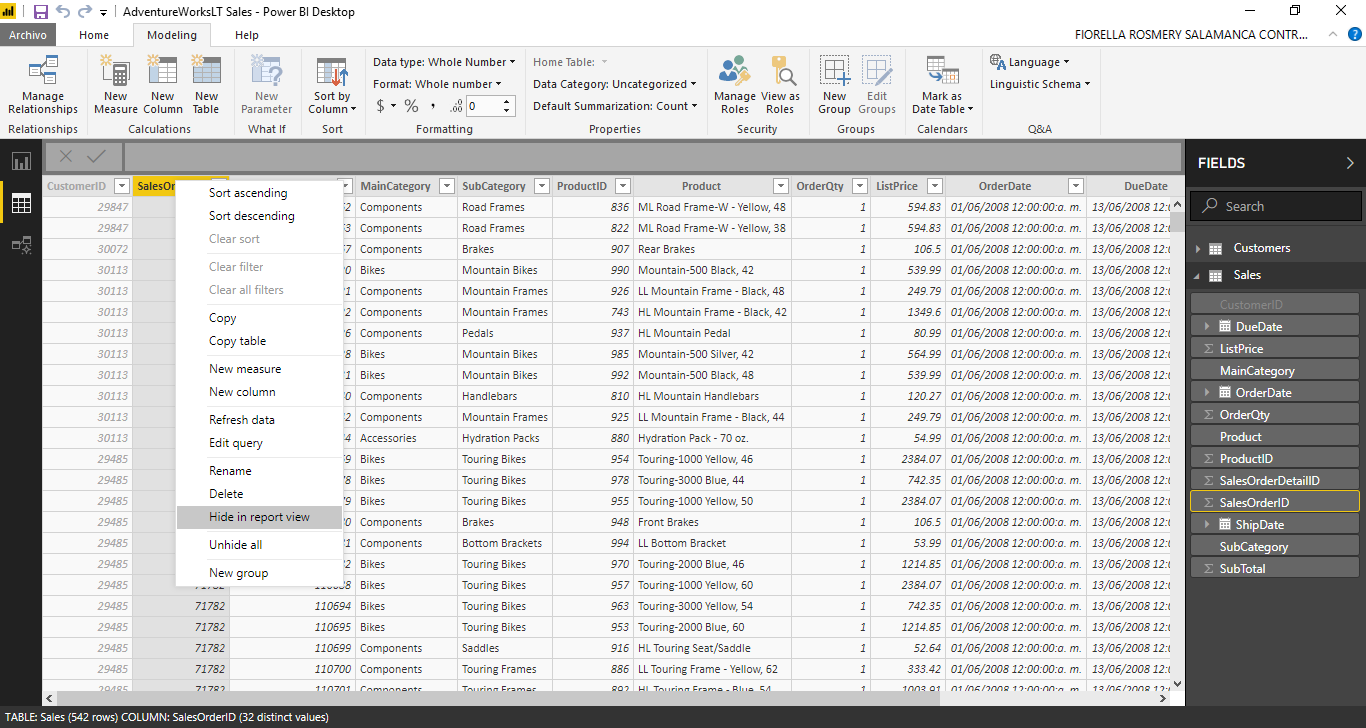
\includegraphics[width=17cm]{./Imagenes/Ejercicio1/Tarea3/25}
	\end{center}	

29. Right-click the SalesOrderDetailID column, and then click Hide in Report View.\\
30. On the Modeling ribbon, in the Calculations group, click New Column, and then in the formula bar, type the following expression and press Enter:\\

\textbf{LineTotal = Sales[OrderQty] * Sales[ListPrice]}

	\begin{center}
	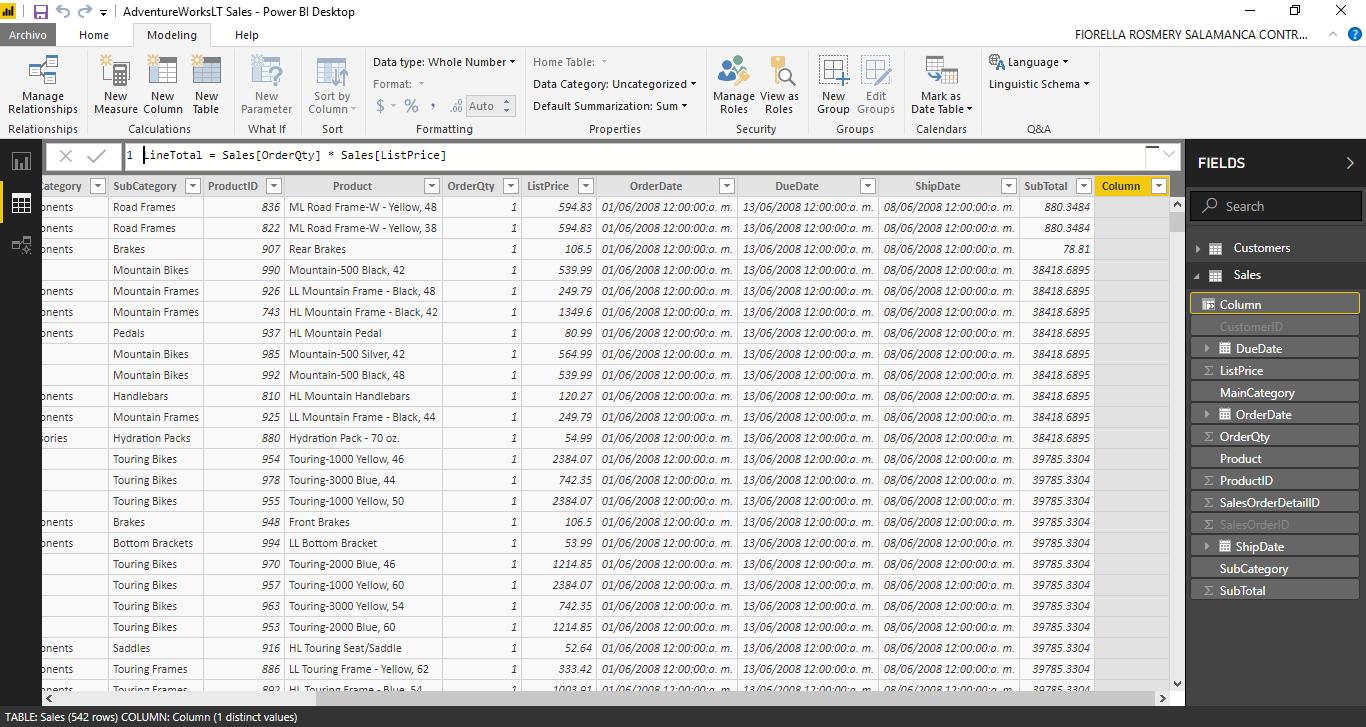
\includegraphics[width=17cm]{./Imagenes/Ejercicio1/Tarea3/26}
	\end{center}	

31. Click the LineTotal column header.\\
32. On the Modeling ribbon, in the Formatting group, click Format: General, point to Currency, and then click \$ English (United States).\\

	\begin{center}
	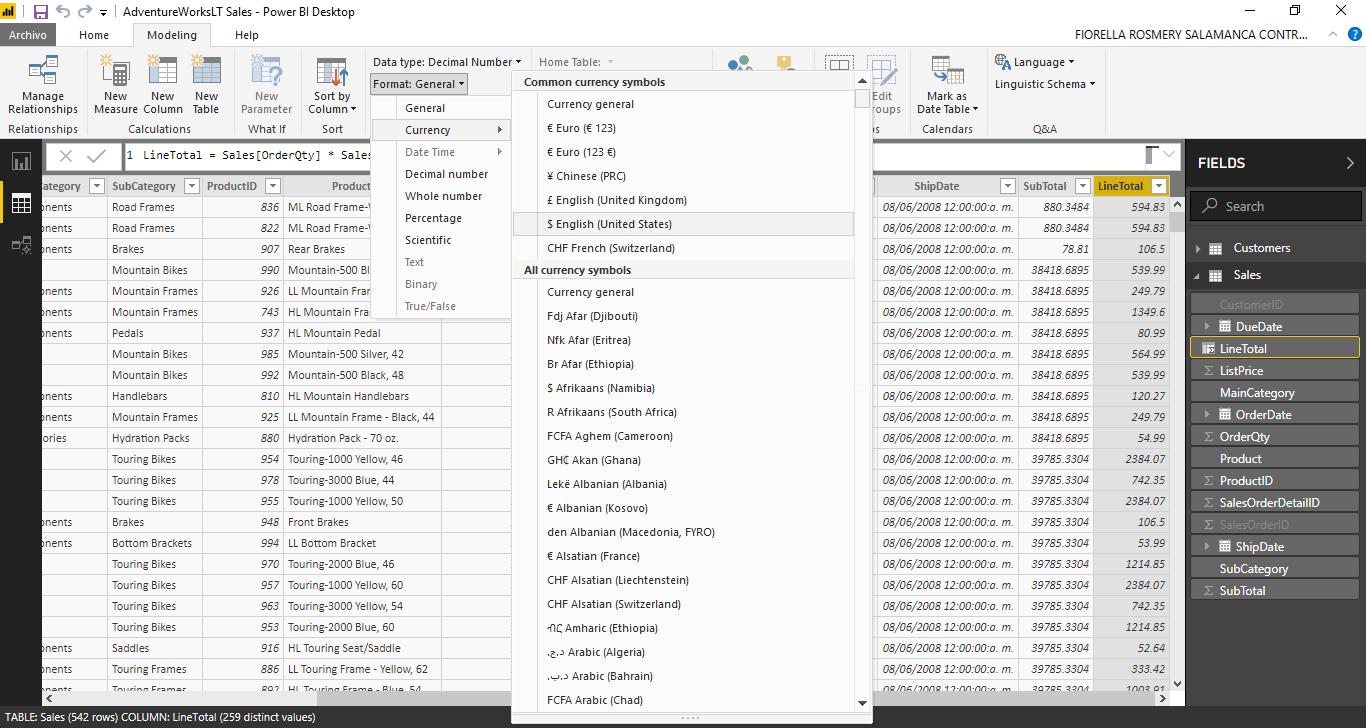
\includegraphics[width=17cm]{./Imagenes/Ejercicio1/Tarea3/27}
	\end{center}	

33. On the Modeling ribbon, in the Calculations group, click New Measure, and then in the formula bar, type the following expression and press Enter:\\

\textbf{TargetSales = SUM('Sales'[LineTotal]) * 1.2}

	\begin{center}
	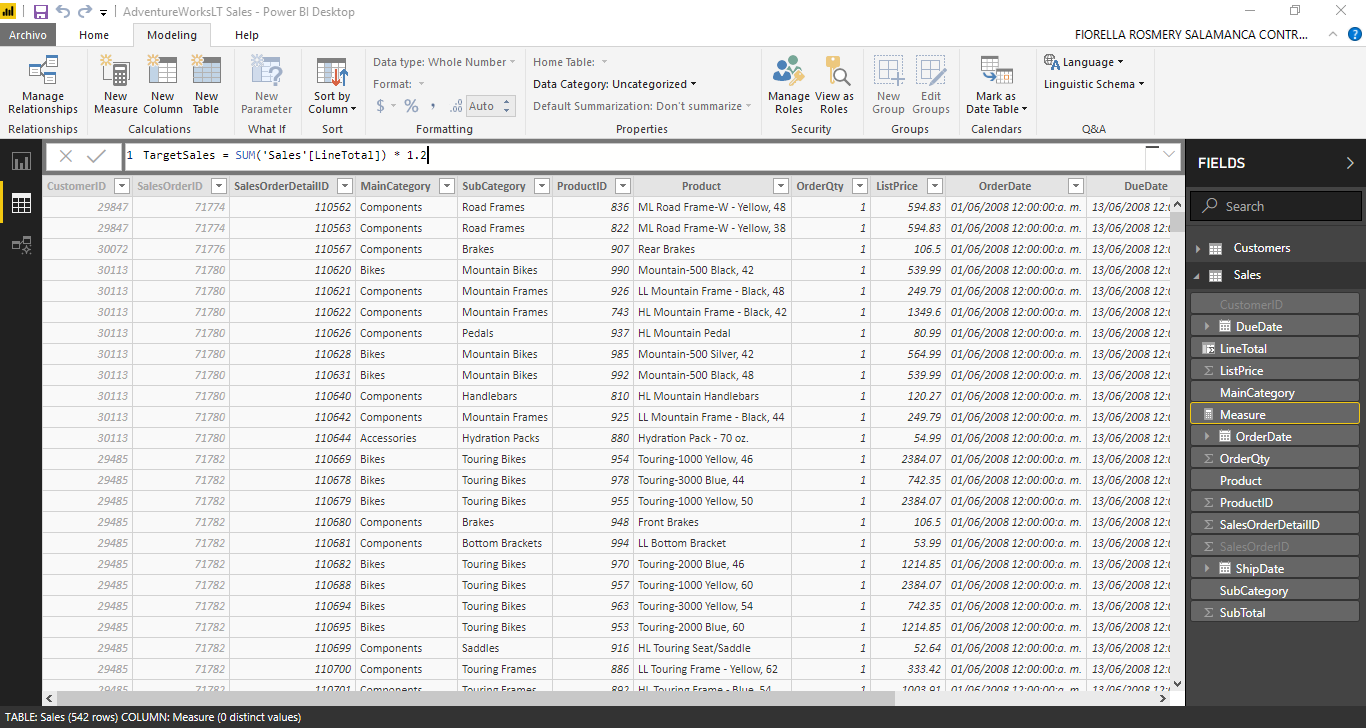
\includegraphics[width=17cm]{./Imagenes/Ejercicio1/Tarea3/29}
	\end{center}	

34. Click Save, and then leave Power BI Desktop open for the next task.
